% Que fue lo que se logr\'o con la experimentaci\'on, incluir tablas y
%  par\'ametros, gr\'aficos si fuera posible, lo m\'as explicativo posible.

 \noindent\begin{tabular*}{\textwidth}{@{\extracolsep{\fill}} ccrrrrrr} \hline
 & & \multicolumn{5}{c}{Restricciones insatisfechas} \\
 \cline{3-7}
 	\textbf{INS} & \textbf{N Clases} & \textbf{OPT}    & $\bar{x}$ & $s$   & $Min$ & $Max$ & $\Delta t$[s] \\ \hline
 	200\_01      &             25    &              0  &  44.18    & 7.033 & 33    & 75    & 27.95     \\
 	200\_02      &             25    &              2  &  39.60    & 6.255 & 26    & 63    & 28.56     \\
 	200\_03      &             25    &              4  &  53.06    & 7.014 & 41    & 90    & 27.82     \\
 	200\_04      &             24    &              7  &  49.44    & 6.405 & 36    & 81    & 27.94     \\
 	200\_05      &             23    &              6  &  33.72    & 5.696 & 25    & 61    & 28.03     \\
 	200\_06      &             23    &              6  &  36.90    & 5.615 & 28    & 58    & 27.93     \\
 	200\_07      &             23    &              0  &  36.13    & 5.620 & 26    & 60    & 27.94     \\
 	200\_08      &             20    &              8  &  31.00    & 4.915 & 24    & 57    & 28.32     \\
 	200\_09      &             24    &             10  &  41.49    & 6.581 & 27    & 71    & 28.29     \\
 	200\_10      &             19    &             19  &  42.90    & 5.339 & 32    & 73    & 28.72     \\ \hline
 	300\_01      &             25    &              0  &  64.33    & 9.293 & 49    & 110   & 46.10     \\
 	300\_02      &             25    &             12  &  65.73    & 8.072 & 53    & 90    & 46.22     \\
 	300\_03      &             25    &             13  &  68.93    & 6.562 & 56    & 99    & 45.79     \\
 	300\_04      &             24    &              7  &  61.77    & 7.450 & 48    & 99    & 45.56     \\
 	300\_05      &             20    &             29  &  106.85   & 8.284 & 97    & 147   & 46.15     \\
 	300\_06      &             25    &              2  &  67.78    & 8.291 & 56    & 104   & 45.47     \\
 	300\_07      &             24    &              0  &  63.90    & 4.603 & 55    & 72    & 46.05     \\
 	300\_08      &             23    &              8  &  59.65    & 11.074& 47    & 96    & 45.55     \\
 	300\_09      &             21    &              7  &  70.55    & 14.982& 57    & 125   & 45.85     \\
 	300\_10      &             19    &             21  &  73.85    & 9.334 & 59    & 103   & 46.10     \\ \hline
 	400\_01      &             25    &              1  &  84.78    & 8.184 & 71    & 123   & 66.68     \\
 	400\_02      &             22    &             16  &  105.4    & 8.429 & 93    & 134   & 66.10     \\
 	400\_03      &             23    &              9  &  86.30    & 7.260 & 75    & 102   & 67.65     \\
 	400\_04      &             26    &             19  &  93.90    & 13.535& 68    & 129   & 65.55     \\
 	400\_05      &             20    &              0  &  74.80    & 8.716 & 60    & 97    & 66.30     \\
 	400\_06      &             23    &              0  &  70.44    & 8.219 & 54    & 95    & 65.58     \\
 	400\_07      &             23    &              4  &  85.05    & 5.371 & 77    & 95    & 66.50     \\
 	400\_08      &             21    &              4  &  90.80    & 5.391 & 76    & 100   & 65.75     \\
 	400\_09      &             24    &              5  &  96.80    & 9.168 & 83    & 123   & 65.75     \\
 	400\_10      &             25    &              0  &  71.50    & 8.393 & 57    & 91    & 65.95     \\ \hline
 \end{tabular*}
\newpage
\begin{figure}[htb!]
	\begin{center}
	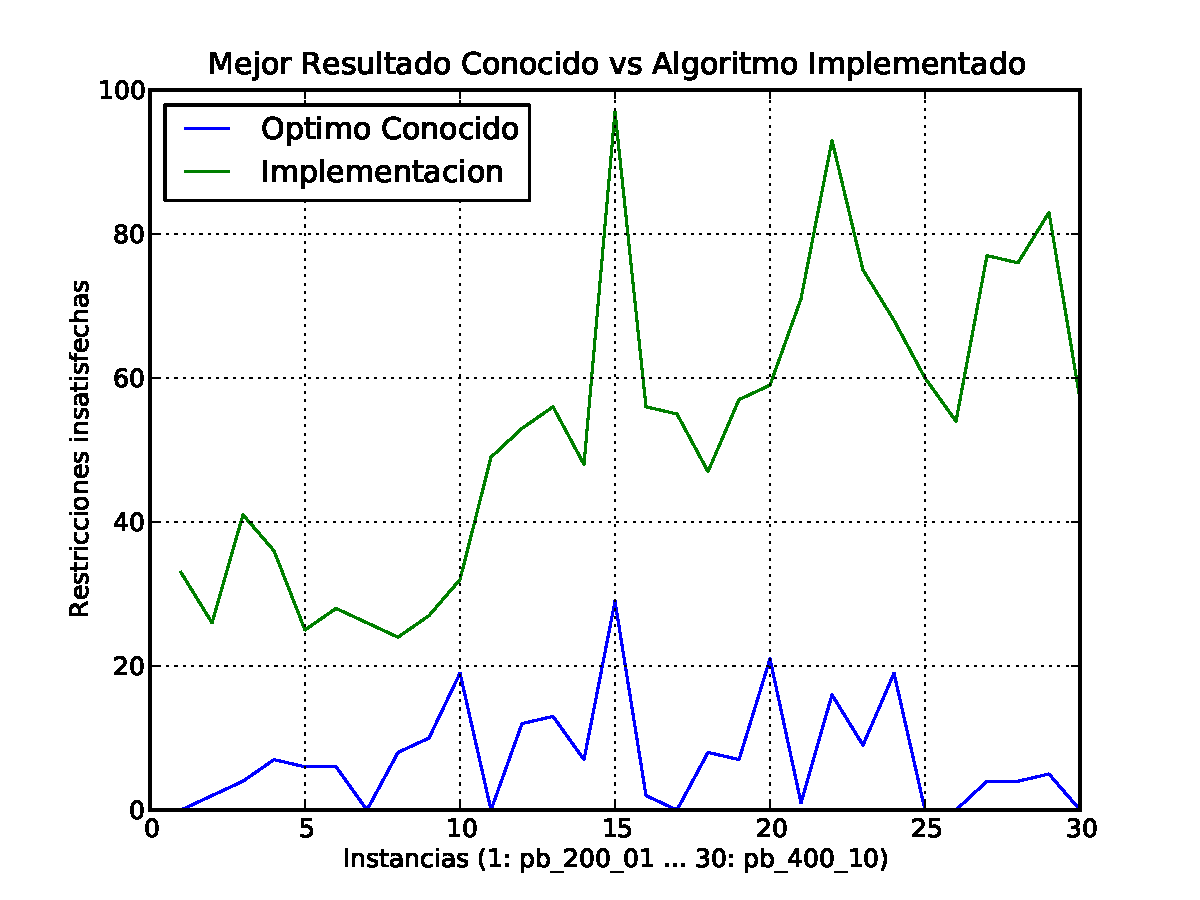
\includegraphics[scale=0.6]{img/fig3}
	\end{center}
	\label{fig:fig3}
	\caption{Mejor óptimo conocido vs Resultados de la implementación}
\end{figure}

En la \textbf{Figura 3} de la sección~\ref{fig:fig3} podemos ver un gráfico que nos muestra la cantidad de las restricciones insatisfechas
por cada instancia $(pb\_200\_01, pb\_200\_02,\ldots, pb\_400\_10$, considerando los mejores óptimos conocidos hasta ahora,
y los resultados de la presente implementación.

